\documentclass[a4paper, 10pt]{article}
\linespread{1.33}
% ┌─────────────────────┐
% │     preamble.tex    │
% └─────────────────────┘

% ══════════ [1] Basic document settings ══════════
\usepackage{fullpage}
\usepackage{geometry}
\geometry{
    top = 2cm,
    bottom = 4.5cm,
    left = 2.5cm,
    right = 2.5cm
}
\usepackage{lastpage}

\usepackage{xcolor}
\usepackage{graphicx}
\usepackage{tikz}
\usepackage{pgfplots}

\usepackage{enumerate}
\usepackage{sectsty}
\subsectionfont{\color{blue}}
\usepackage{enumitem}
\usepackage{array}
\newcolumntype{P}[1]{>{\centering\arraybackslash}p{#1}}

\usepackage{fourier-orns}
\usetikzlibrary{decorations.text}
\pgfplotsset{compat = newest}
\newcommand{\seprule}{
    \vspace*{1.5em}
    \vspace{-8pt}\hrulefill
    \raisebox{-2.1pt}{\quad\decofourleft\decotwo\decofourright\quad}\hrulefill
    \vspace*{1.5em}
}

\usepackage{hyperref}
\hypersetup{
  colorlinks=true,
  linkcolor=blue,
  linkbordercolor={0 0 1},
  urlcolor=blue
}

\usepackage{fancyhdr}
\usepackage[]{mdframed}

\renewcommand{\thesubsection}{\S{} \arabic{section}.\arabic{subsection}}

% ══════════ [2] Math packages ══════════
\usepackage{amsmath}
\usepackage{amsthm}
\usepackage{amsfonts}
\usepackage{amssymb}
\usepackage{amscd}
\usepackage{mathrsfs}
\usepackage{cancel}

% ══════════ [3] Miscellaneous & Fonts ══════════
\setlength{\parindent}{0.0in}
\setlength{\parskip}{0.05in}
\renewcommand{\footrulewidth}{0.4pt}

\usepackage{mathpazo}
\usepackage{domitian}
\usepackage[T1]{fontenc}
\let\oldstylenums\oldstyle
\setmonofont[Scale = 0.8]{DejaVu Sans Mono}

% ══════════ [4] amsthm setup ══════════

\newtheorem{theorem}{Theorem}[section]
\newtheorem{corollary}[theorem]{Corollary}
\newtheorem{lemma}[theorem]{Lemma}

\theoremstyle{definition}
\newtheorem{definition}[theorem]{Definition}

\theoremstyle{remark}
\newtheorem*{remark}{Remark}

\theoremstyle{definition}
\newtheorem{obs}[theorem]{Observation}

\theoremstyle{definition}
\newtheorem{exercise}[theorem]{Exercise}
\newmdtheoremenv[innertopmargin = 8pt,
                 innerbottommargin = 10pt]{exer}[theorem]{Exercise}

\theoremstyle{definition}
\newtheorem{example}[theorem]{Example}
% ┌─────────────────────┐
% │   usercommand.tex   │
% └─────────────────────┘

% ══════════ [1] short-hand notations ══════════
\newcommand{\mbf}{\mathbf}
\newcommand{\mrm}{\mathrm}
\newcommand{\mca}{\mathcal}
\newcommand{\msc}{\mathsc}
\newcommand{\mbb}{\mathbb}
\newcommand{\msf}{\mathsf}

\newcommand{\tbf}{\textbf}
\newcommand{\tit}{\textit}

\newcommand{\eps}{\epsilon}
\newcommand{\kB}{k_{\mathrm{B}}}
\def\dbar{{\mathchar'26\mkern-12mu d}}
\newcommand{\contradiction}{\ensuremath{{\Rightarrow\mspace{-2mu}\Leftarrow}}}
\newcommand{\im}{\mathrm{im}\,}
\renewcommand{\d}{\mathrm{d}}

\renewcommand\qedsymbol{$\blacksquare$}

\newcommand\lecturenumber{04}
\newcommand\lecturedate{Nov 1, 2024}

\pagestyle{fancyplain}
\headheight 40pt
\lhead{Lecture \lecturenumber\\CNBC Deep Learning Subgroup}
\rhead{Riemannian Geometry for Deep Learning \\\lecturedate}
\cfoot{Fall 2024, SNU}
\rfoot{\small\thepage}
\headsep 1.5em

\begin{document}
\setcounter{section}{3}
\setcounter{subsection}{0}
\setcounter{theorem}{0}

\section{Manifolds: Definitions}

\subsection{Topological Spaces}

\begin{definition}[Topological space]
    Let $X$ be any set and $\mca{T} = \{ U_{i} \,:\, i \in I \}$ be a \tit{collection} of subsets of $X$. The pair $(X, \mca{T})$ is a \tbf{topological space} if $\mca{T}$ satisfies
    \begin{itemize}
        \item[(i)] $\varnothing \in \mca{T}$ and $X \in \mca{T}$.
        \item[(ii)] $\displaystyle{\bigcup_{j \in J} U_{j} \in \mca{T}}$ where $J$ is a subcollection of $I$. Here, union can be infinite.
        \item[(iii)] $\displaystyle{\bigcap_{k \in K} U_{k} \in \mca{T}}$ where $K$ is a \tit{finite} subcollection of $I$.
    \end{itemize}
    Here $U_{i}$ are called the \tbf{open set} and $\mca{T}$ is said to give a \tbf{topology} to $X$.
\end{definition}

\begin{remark}
    Do you remember the definition of \tit{open sets} in analysis?
    \begin{itemize}
        \item[(i)] $U$ is \tit{open} if all point of $U$ is an \tit{interior} point of $U$.
        \item[(ii)] $x \in U$ is an \tit{interior} point of $U$ if there exists some \tit{neighborhood} $N(x)$ of $x$ such that $N(x) \in U$.
        \item[(iii)] The \tit{neighborhood} of $x$ with radius $r$ is $N_{r}(x) = \{ y \in U \,|\, d(x,y) < r \}$.
    \end{itemize}
    The definition of open set requires the concept of \tbf{metric space}.
\end{remark}

\begin{example}
    Example of topologies.
    \begin{itemize}
        \item[(1)] Let $X$ be a set and $\mca{T}$ be the collection of all subsets of $X$. This gives \tbf{discrete topology} to $X$.
        \item[(2)] Let $X$ be a set and $\mca{T} = \{ \varnothing, X \}$. This gives \tbf{trivial topology} to $X$.
        \item[(3)] Let $X = \mbb{R}$ and $\mca{T}$ be all open intervals and their unions. This defines a \tbf{usual topology} to $\mbb{R}$. This can be extended to $\mbb{R}^{n}$.
    \end{itemize}
\end{example}

\begin{remark}
    A subset $A$ of $X$ is \tit{closed} if its complement in $X$ is an open set $X - A \in \mca{T}$.
\end{remark}

\seprule

\begin{definition}[Metric]
    A metric $d \,:\, X \times X \rightarrow \mbb{R}$ is a map that satisfies
    \begin{itemize}
        \item[(i)] $d(x,y) = d(y,x)$
        \item[(ii)] $d(x,y) \geq 0$ and $d(x,y) = 0 \;\Longleftrightarrow\; x = y$
        \item[(iii)] $d(x,y) + d(y,z) \geq d(x,z)$ (triangle inequality)
    \end{itemize}
    for $x, y, z \in X$.
\end{definition}
\newpage

% ===== ===== ===== ===== ===== ===== ===== ===== ===== ===== ===== =====

\begin{definition}[Metric space and metric topology]
    If $X$ is endowed with a metric $d$, $X$ is made into a topological space whose open sets are given by \tit{open discs}, $U_{\epsilon}(x) = \{ y \in X \,|\, d(x,y)<\epsilon \}$ and their possible unions. Then $\mca{T}$ is called a \tbf{metric topology} and $(X, \mca{T})$ a \tbf{metric space}.
\end{definition}

\begin{definition}[Relative topology]
    Let $(X, \mca{T})$ be a topological space and $A \subseteq X$. Then $\mca{T} = \{U_{i} \,:\, i \in I \}$ induces the \tbf{relative topology} in $A$ by
    \[ \mca{T}' = \{ U_{i} \cap A \,|\, U_{i} \in \mca{T} \} \]
\end{definition}

\begin{definition}[Continuous map]
    Let $X$ and $Y$ be topological spaces. A map $f \,:\, X \rightarrow Y$ is \tbf{continuous} if the inverse image of an open set in $Y$ is an open set in $X$.
\end{definition}

\begin{definition}[Neighborhood]
    $N$ is a \tbf{neighborhood}\footnote{The neighborhood needs not be an open set.} of a point $x \in X$ if $N \subseteq X$ and $N$ contains at least one open set $U_{i}$ which contains $x$.
\end{definition}

\begin{definition}[Hausdorff space]
    A topological space $(X, \mca{T})$ is a \tbf{Hausdorff space} if: for $x, x' \in X$, there exist neighbors $U_{x}$ of $x$ and $U_{x'}$ of $x'$ such that $U_{x} \cap U_{x'} = \varnothing$.
\end{definition}

\begin{exercise}
    Prove the following statements.
    \begin{itemize}
        \item[(1)] $\mbb{R}$ with the usual topology is a Hausdorff space.
        \item[(2)] Every metric space is a Hausdorff space.
    \end{itemize}
\end{exercise}

\subsection{Introductory Topology}

\begin{definition}[Compactness]
    Let $X$ be a set.
    \begin{itemize}
        \item[(1)] A family $\{A_{i}\}$ of subsets of $X$ is called a \tbf{covering} of $X$ if $\displaystyle{\bigcup_{i \in I}A_{i} = X}$. If all the $A_{i}$ happen to be the open sets of the topology $\mca{T}$, the covering is called an \tbf{open covering}.
        \item[(2)] The set $X$ is \tbf{compact} if: for every open covering $\{ U_{i} \,:\, i \in I \}$, there exists finite subcovering $\{ U_{j} \,:\, j \in J \subseteq I \}$.
    \end{itemize}
\end{definition}

\begin{theorem}[Heine-Borel theorem]
    For a subset $X \subseteq \mbb{R}^{n}$, $X$ is compact if and only if $X$ is closed and bounded.
\end{theorem}
\begin{remark}
    A point in $\mbb{R}^{n}$ is compact.
\end{remark}
\newpage

% ===== ===== ===== ===== ===== ===== ===== ===== ===== ===== ===== =====

\begin{definition}[Connectedness]
    \hphantom{.}
    \begin{itemize}
        \item[(a)] A topological space $X$ is \tbf{connected} if it cannot be written as $X = X_{1} \cup X_{2}$ where $X_{1}$ and $X_{2}$ are both open and $X_{1} \cap X_{2} = \varnothing$.
        \item[(b)] A topological space is \tbf{arcwise connected} if for any points $x, y \in X$ there exists a continuous map $f \,:\, [0,1] \rightarrow X$ such that $f(0) = x$ and $f(1) = y$.
        \item[(c)] A \tbf{loop} in a topological space $X$ is a continuous map $f \,:\, [0,1] \rightarrow X$ such that $f(0) = f(1)$. If any loop in $X$ can be continuously shrunk to a point, then $X$ is called \tbf{simply connected}.
    \end{itemize}
\end{definition}

\begin{example}
    \hphantom{.}
    \begin{itemize}
        \item[(a)] $\mbb{R}$ is arcwise connected while $\mbb{R}-\{0\}$ is not. Meanwhile, both $\mbb{R}^{n}$ and $\mbb{R}^{n} - \{0\}$ are arcwise connected for $n \geq 2$.
        \item[(b)] $S^{n}$ is arcwise connected. $S^{1}$ is not simply connected while  $S^{n}\,(n\geq 2)$ is simply connected. The $n$-dimensional torus
        \[ T^{n} = \underbrace{S^{1} \times \cdots \times S^{1}}_{n} \]
        is arcwise connected but not simply connected.
        \item[(c)] $\mbb{R}^{2} - \mbb{R}$ is not arcwise connected. $\mbb{R}^{2} - \{0\}$ is arcwise connected but not simply connected. However, $\mbb{R}^{3}-\{0\}$ is both arcwise connected and simply connected.
    \end{itemize}
\end{example}

\seprule

\tbf{Topology} is about classifying the spaces (are they equal or different?). In topology, two figures are \tit{equivalent} if it can be deformed continuously from one to the other.
\begin{definition}[Homeomorphisms]
    Let $X_{1}$ and $X_{2}$ be topological spaces. A map $f \,:\, X_{1} \rightarrow X_{2}$ is a \tbf{homeomorphism} if it is continuous and has an inverse $f^{-1} \,:\, X_{2} \rightarrow X_{1}$ which is also continuous. Then, $X_{1}$ and $X_{2}$ are \tbf{homeomorphic}. In other words,
    \[ \exists\, f\,:\, X_{1} \rightarrow X_{2},\; g\,:\, X_{2} \rightarrow X_{1} \quad\text{s.t.}\quad f\circ g = \mrm{id}_{X_{2}}\;\text{and}\;g\circ f = \mrm{id}_{X_{1}} \]
\end{definition}

\begin{remark}
    Homeomorphisms give equivalence relations, which divide all topological spaces into equivalence classes(Is it possible to deform one space into other by a homeomorphism).
\end{remark}
\newpage

% ===== ===== ===== ===== ===== ===== ===== ===== ===== ===== ===== =====

\begin{exer}
    \hphantom{.}
    \begin{itemize}
        \item[(1)] $X = \{ 1,\, 1/2,\, \cdots,\, 1/n \} \subseteq \mbb{R}$ is not closed in $\mbb{R}$.
        \item[(2)] $Y = X \cup \{0\}$ is closed in $\mbb{R}$.
        \item[(3)] $Y$ is compact.
    \end{itemize}
\end{exer}

\begin{proof}
    \hphantom{.}
    \begin{itemize}
        \item[(1)] Firstly, $X$ is not open because it is a set of isolated points. Considering the complement of $X$,
        \[ (-\infty, 0] \cup (1, \infty) \cup (1/2, 1) \cup (1/3, 1/2) \cup \cdots  \]
        Since $\mbb{R}-X$ contains \tit{accumulation point} 0, $(-\infty, 0]$ makes it not open. Therefore, $X$ is not closed.
        \item[(2)] Trivial from (1).
        \item[(3)] Heine-Borel theorem (theorem 4.11).
    \end{itemize}
\end{proof}

\begin{exer}
    Show that these two figures are homeomorphic. Show that those linked rings are separable (or deformable into separated rings) in $\mbb{R}^{4}$.
\end{exer}

\begin{figure}[htbp!]
    \centering
    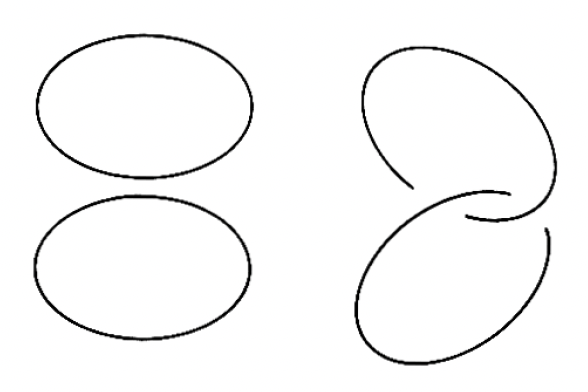
\includegraphics[width=0.3\linewidth]{../images/lecture04/4_01.png}
\end{figure}

\begin{proof}
    Let two rings in separated and linked forms be (A, B) and (A', B'), respectively. If we take homeomorphisms from A to A' and B to B' and combine them, separated rings and linked rings are homeomorphic.

    \tbf{Existence of homotopy.} Consider a homotopy $\{0, 1\} \times (S^{1} \sqcup S^{1}) \rightarrow \mbb{R}^{4}$, where the image of $(0,\bullet,\bullet)\,:\, S^{1}\sqcup S^{1} \rightarrow \mbb{R}^{4}$ denotes separated rings and $(1,\bullet,\bullet) \,:\, S^{1} \sqcup S^{1} \rightarrow \mbb{R}^{4}$ denotes linked rings. Assuming separated and linked rings are embedded in $\mbb{R}^{3} \times \{0\}$, we can use the fourth coordinate to lift one of the two rings in separated rings to the $(\bullet, \bullet, \bullet, 1)$ plane. Move it over to the corresponding ring on the linked ring and move it back to $(\bullet, \bullet, \bullet, 0)$ plane.
\end{proof}

\end{document}
